\section{Opisać rozszerzony algorytm Euklidesa znajdowania NWD.}
Dla danych \( a, b > 0 \) algorytm zwraca \( d = \gcd(a,b) \) oraz liczby całkowite \( s \) i \( t \), które spełniają \( d = s\cdot a + t\cdot b \).

\begin{greyframe}
    Algorytm:
    \begin{enumerate}
        \item Jeśli \( a < b \), zamień \( a \) z \( b \).
        \item Jeśli \( b = 0 \), zwróć \( d = a \) i parę \( (1,0) \).
        \item Oblicz \( a = q \cdot b + r \).
        \item Wywołaj \( \gcd(b,r) \), otrzymując \( d \) i parę \( (s', t') \) taką, że \( s'\cdot b + t' \cdot r = d \).
        \item Zwróć \( d \) i parę \( (t', s' - q \cdot t') \).
    \end{enumerate}
\end{greyframe}

\vspace{1em}\noindent
\textit{Algorytm zwraca poprawne \( d = \gcd(a, b) \).}
\begin{proof}
    Wystarczy pokazać, że \( \gcd(a, b) = \gcd(b, r) \), jeśli \( a = q \cdot b + r \). Niech \( d = \gcd(a, b) \).
    \[
        a = 0 \pmod{d}
    \]
    \[
        b = 0 \pmod{d}
    \]
    \[
        r = a - q \cdot b = 0 \pmod{d}
    \]
\end{proof}
\textit{Algorytm zwraca poprawne \( (s, t) \).}
\begin{proof}[Dowód -- indukcja po mniejszym argumencie]
    Jako krok bazowy indukcji po \( a, b \) sprawdzamy przypadek \( b = 0 \), rzeczywiście \( a \cdot 1 + 0 = \gcd(a, 0) \). \\
    Niech \( a = q \cdot b + r \). Korzystając z tego, że \( \gcd(a, b) = \gcd(b, r) = d \), otrzymujemy:
    \[
        b \cdot s' + r \cdot t' = d,
    \]
    \[
        b \cdot s' + (a - q \cdot b) \cdot t' = d,
    \]
    czyli \( s = t', \ t = s' - q \cdot t' \), co było do pokazania.
\end{proof}
Zatem algorytm w konstruktywny sposób dowodzi tożsamości B\'ezout.

Własności algorytmu:
\begin{enumerate}
    \item Liczba iteracji: co najwyżej \( \log_{\phi} a \), gdzie \( \phi = \frac{1 + \sqrt{5}}{2} \)
    \item Złożoność: \( \bigO(\log^2 a) \)
    \item \( \abs{s} \leq b \), \( \abs{t} \leq a \)
\end{enumerate}
Ad 1. Żeby obliczenie \( \gcd(a, b) \) wymagało \( k \) kroków, potrzeba \( a \geq F_{k+2} \), \( b \geq F_{k+1} \) -- dowód przez indukcję po \( k \). \\
Ad 2. Przy każdym wywołaniu rekurencyjnym przynajmniej jeden z argumentów zmniejsza się o połowę: \\
Jeśli \( b \leq \frac{a}{2} \), to \( r < b < \frac{a}{2} \). \\
Jeśli \( b > \frac{a}{2} \), to \( r = a - b < \frac{a}{2} \). \\
Złożoność operacji w kroku rekursji  to \( \bigO(\log a) \), więc cały algorytm ma złożoność \( \bigO(\log^2 a) \).

\section{Opisać binarny algorytm Euklidesa znajdowania NWD.}
Dla danych \( a,b > 0 \) algorytm zwraca \( \gcd(a,b) \), wykonując tylko odejmowanie i operacje binarne.

\begin{greyframe}
    Algorytm:
    \begin{enumerate}
    \item Jeśli \( a < b \), zamień \( a \) i \( b \).
    \item Jeśli \( b = 0 \), zwróć \( d = a \).
    \item Jeśli \( 2 \mid a \) i \( 2 \nmid b \), zwróć \( \gcd\pars{\frac{a}{2}, b} \),
    \item Jeśli \( 2 \nmid a \) i \( 2 \mid b \), zwróć \( \gcd\pars{a, \frac{b}{2}} \),
    \item Jeśli \( 2 \mid a \) i \( 2 \mid b \), zwróć \( 2 \cdot \gcd\pars{\frac{a}{2}, \frac{b}{2}} \),
    \item Jeśli \( 2 \nmid a \) i \( 2 \nmid b \), zwróć \( \gcd\pars{b, a - b} \).
    \end{enumerate}
\end{greyframe}

\vspace{1em}\noindent
\textit{Algorytm zwraca poprawne \( d = \gcd(a, b) \).}
\begin{proof}
    Jeśli któryś z argumentów jest nieparzysty (przypadki 3 i 4), to \( 2 \nmid \gcd(a, b) \), dlatego możemy podzielić parzysty argument przez 2. \\
    Jeśli oba argumenty są parzyste (przypadek 5), to \( d = \gcd(a, b) \) też jest parzyste, ponieważ inaczej \( 2 \cdot d \) dzieliłoby obie liczby, co byłoby sprzeczne z tym, że \( d \) jest największym dzielnikiem.
    Dlatego możemy wydzielić 2 i obliczyć \( 2 \cdot \gcd\pars{\frac{a}{2}, \frac{b}{2}} \). \\
    Jeśli obie liczby są nieparzyste, to obliczamy \( d = \gcd(b, a - b) = \gcd(a, b) \), ponieważ:
    \[
        a \equiv 0 \ \mod \ d
    \]
    \[
        b \equiv 0 \ \mod \ d
    \]
    \[
        a - b \equiv 0 \ \mod \ d
    \]
\end{proof}

W każdym z przypadków od 3 do 5, co najmniej jeden z argumentów zmniejsza się o połowę. Takich wywołań jest więc co najwyżej logarytmicznie wiele.
Pozostaje do przeanalizowania przypadek 6. Ponieważ \( a \) i \( b \) są nieparzyste, to \( a - b \) jest parzyste, więc w kolejnym wywołaniu wykona się przypadek 3 lub 4. Czyli któryś z argumentów zmniejszy się o połowę w co najwyżej dwóch krokach.
To dowodzi złożoności \( \bigO(\log(a) \cdot M(a)) \), gdzie \( M(a) \) to koszt odejmowania i~operacji bitowych, który jest liniowy od długości zapisu liczb.

\section{Opisać algorytmy szyfrowania RSA i Elgamal oraz na czym polega trudność ich łamania.}
Algorytmy RSA i Elgamal są asymetryczne, czyli wykorzystują jawną funkcję szyfrującą \( E \) (klucz publiczny) i tajną funkcję deszyfrującą \( D \) (klucz prywatny).
Najważniejszym założeniem jest, że nie potrafimy efektywnie odtworzyć klucza prywatnego z publicznego. Dodatkowo zakładamy, że problem Factoring nie jest w klasie BPP.

\subsection{Algorytm RSA}
\begin{greyframe}
    Algorytm RSA:
    \begin{enumerate}
        \item Oblicz \( N = p \cdot q \) dla wybranych liczb pierwszych \( p \), \( q \). \\
        Wtedy \( \varphi(N) = (p-1) \cdot (q-1) \).
        \item Wybierz \( e \) względnie pierwsze z \( \varphi(N) \). Oblicz \( d \) takie, że  \( e\cdot d = 1 \pmod{\varphi(N)} \).
        \item Zdefiniuj \( E(x) = x^e \pmod{N} \) oraz \( D(x) = x^d \pmod{N} \). Kluczem publicznym \\ jest \( (e, n) \).
    \end{enumerate}
\end{greyframe}

Ad 1. Zamiast \( \varphi(N) \) można użyć (rozwiązanie często stosowane) funkcji Carmichaela
\[
    \lambda(N) = \lcm(p - 1, q - 1)
\]
Funkcja \( \lambda \) znajduje najmniejszą liczbę całkowitą \( x \) taką, że \( x^{\lambda(N)} = 1 \pmod{N} \) dla każdego \( x \) względnie pierwszego z \( N \).
Wybór \( \lambda(N) \) zamiast \( \varphi(N) \) nie zmniejsza bezpieczeństwa, a daje zazwyczaj mniejszy wykładnik. \\
Ad 2. Do znalezienia liczby \( d \) można użyć rozszerzonego algorytmu Euklidesa:
\[
    e \cdot s + \varphi(N) \cdot t = 1
\]
\[
    s + \varphi(N) \cdot t \cdot e^{-1} = e^{-1} \pmod{\varphi(N)}
\]
\[
    d = s = e^{-1} \pmod{\varphi(N)}
\]
Dlaczego deszyfrowanie działa? \\
Rząd grupy multiplikatywnej modulo \( N \) jest równy \( \varphi(N) \), więc dla każdego \( x \) względnie pierwszego z \( N \) zachodzi
\[
    (x^{e})^d = x^{ed} = x^{k \cdot \varphi(N) + 1} = x,
\]
ponieważ \( e \cdot d = 1 \pmod{\varphi(N)} \), a na mocy twierdzenia Lagrange'a \( x^{\varphi(N)} = 1 \).

Szyfrowanie RSA można złamać, jeśli wyznaczy się liczby \( p \) i \( q \), czyli pozna się rozkład \( N \) na czynniki pierwsze.
Można wtedy obliczyć \( \varphi(N) \) i \( d \) algorytmem Euklidesa. Dlatego tak ważne jest założenie o dużej trudności problemu Factoring.
W tym dniu (18.05.2025), nie ma ani dowodu na to, że algorytm rozkładu na czynniki pierwsze nie istnieje, ani dowodu NP-zupełności problemu Factoring.

\subsection{Algorytm Elgamal}
\begin{greyframe}
    Algorytm Elgamal:
    \begin{enumerate}
        \item Wybierz jakąś grupę \( G \) (np. grupę multiplikatywną ciała \( \mathbb{F}_q \)) i element \( g \in G \) \\ (najlepiej generator).
        \item Wylosuj liczbę \( x \in \set{1, \ldots, \abs{G}-1} \).
        \item Klucz publiczny to \( (g,g^x) \), a klucz prywatny to \( (g,x) \).
        \item Szyfrowanie wiadomości \( M \): wylosuj liczbę \( y \), wyślij \( (g^y, M \cdot g^{xy}) \). 
    \end{enumerate}
\end{greyframe}
Otrzymawszy \( (g^y, \ M \cdot g^{xy}) \) i znając klucz prywatny \( x \), można łatwo obliczyć \( g^{xy} \), czyli też odtworzyć \( M = \pars{M \cdot g^{xy}} \cdot g^{-xy} \).
Gdyby odszyfrowanie \( M \) było łatwe, to również problem Diffiego-Hellmana byłby rozwiązywalny, a nie jest.

\newpage
\section{Opisać metodę klucza jednorazowego Vernama, trudność jej łamania i praktyczne zastosowanie.}
Osoby A i B mają bezpieczny kanał komunikacji do przesyłania kluczy i niechroniony kanał do zwykłej komunikacji. Osoba A chce przesłać osobie B ciąg bitów \( M \).
Szyfruje go kluczem \( k \) o~takiej samej długości za pomocą bitowej operacji XOR: \( E(M) = M \oplus k \).
Osoba A przesyła bezpiecznym kanałem wartość \( k \) i normalnym kanałem wartość \( E(M) \). Żeby osoba B mogła odczytać \( M \) wystarczy, że obliczy \( E(E(M)) \), ponieważ XOR jest łączny:
\[
	(M \oplus k) \oplus k = M \oplus (k \oplus k)  = M \oplus 0 = M
\]

Przy ,,naprawdę losowym'' \( k \) każdy wynik szyfrowania jest równie prawdopodobny, więc zaszyfrowana wiadomość ma takie same właściwości, co gdyby wylosować osobno każdy bit.

Pozostaje jedno uzasadnione zastrzeżenie -- jeśli musimy mieć sposób na bezpieczne przesłanie klucza o długości \( \abs{M} \), równie dobrze można po prostu przesłać \( M \).
Jednak metoda może być przydatna, jeśli potrzebne jest awaryjne, jednorazowe przesłanie zaszyfrowanej wiadomości i~korespondenci wcześniej mieli okazję wymienić się odpowiednio długim kluczem.

\section{Zdefiniować problemy Primes oraz Factoring i~podać ich umiejscowienie w klasach złożoności.}
\subsection{Primes}
\textbf{Wejście:} Liczba \( p \) \\
\textbf{Problem:} Czy \( p \) jest liczbą pierwszą? \\
\textbf{Klasa złożoności:} P

Primes \( \in \) coNP: \\
Jeśli otrzymamy od wyroczni \( d \) potencjalny dzielnik \( p \), możemy w wielomianowym czasie sprawdzić, czy \( d \) rzeczywiście jest dzielnikiem i odpowiedzieć NIE na pytanie o pierwszość.

Primes \( \in \) NP: \\
Korzystamy z tego, że \( \integer_p^* \) ma rząd równy \( p-1 \) wtedy i tylko wtedy, gdy \( p \) jest pierwsze. \\
Jeśli otrzymamy od wyroczni \( g \), generator \( \integer_p^* \) i rozkład \( p-1 = p_1^{\alpha_1} \cdots p_s^{\alpha_s} \), możemy:
\begin{itemize}
    \item rekurencyjnie sprawdzić pierwszość \( p_i \) i poprawność rozkładu,
    \item sprawdzić, czy \( g^{p-1} = 1 \pmod{p} \),
    \item sprawdzić, czy \( g^{\frac{p-1}{p_i}} \neq 1 \pmod{p} \).
\end{itemize}
Jeżeli wszystkie z powyższych warunków są spełnione, to odpowiedzią jest TAK.

\newpage
Primes \( \in \) BPP: \\
Dowodem jest algorytm Millera-Rabina, który myli się przy odpowiedzi TAK z prawdopodobieństwem nie większym niż \( \frac{1}{2} \).

Primes \( \in \) P: \\
Dowodem jest algorytm Agrawala-Kayala-Saxena (AKS).

\subsection{Factoring}
\textbf{Wejście:} Liczby \( n,\; k \) \\
\textbf{Problem:} Czy istnieje nietrywialny dzielnik \( n \) mniejszy lub równy \( k \)? \\
\textbf{Klasa złożoności:} NP \( \cap \) coNP?

Factoring \( \in \) NP: \\
Jeśli otrzymamy od wyroczni \( 2 \leq d \leq k \) potencjalny dzielnik \( n \), możemy w wielomianowym czasie sprawdzić, czy \( d \) rzeczywiście jest dzielnikiem i odpowiedzieć TAK.

Factoring \( \in \) coNP: \\
Otrzymujemy od wyroczni rozkład liczby \( n \) na czynniki pierwsze \( n = p_1^{\alpha_1} \cdots p_s^{\alpha_s} \). Po sprawdzeniu poprawności rozkładu odpowiadamy \( (p_1 \leq k) \) ? TAK : NIE, gdzie \( p_1 \) to najmniejszy z~dzielników.

Na ten moment nie wiadomo nic więcej.

\section{Podać efektywną metodę znalezienia liczby pierwszej o zadanej liczbie bitów.}
Dla zadanej liczby \( k \) chcemy znaleźć liczbę pierwszą \( p \in \brackets{2^k, 2^{k+1}-1} \).

Liczby pierwsze są dość gęsto upakowane -- w przedziale od 1 do \( n \) jest około \( \frac{n}{\log n} \) liczb pierwszych.
Zatem w przedziale \( \brackets{2^k, 2^{k+1}-1} \) jest ich około
\[
    \frac{2^{k+1} - 1}{k+1} - \frac{2^{k} - 1}{k} = \frac{2^k\pars{1-\frac{1}{k}} - 1}{k+1} = \Theta\pars{\frac{2^k}{k}}
\]

Możemy więc po prostu losować liczbę całkowitą \( p \) z przedziału \( \brackets{2^k, 2^{k+1}-1} \), dopóki nie trafi się liczba pierwsza.
Skoro w przedziale jest \( \Theta\pars{2^k} \) liczb całkowitych, z których \( \Theta\pars{\frac{2^k}{k}} \) jest liczbami pierwszymi, to w oczekiwaniu po \( \bigO(k) \) losowaniach trafimy na liczbę pierwszą.
Sprawdzanie, czy liczba jest pierwsza, wykonuje się w czasie \( \bigO\pars{k^3} \), więc oczekiwana złożoność algorytmu losowania liczby pierwszej to \( \bigO\pars{k^4} \).

\section{Opisać efektywną implementację działań arytmetycznych w ciele \( \integer_p/(w) \).}
Jeśli \( w \) jest wielomianem nierozkładalnym stopnia \( n \), to elementy
elementy \( \integer_p/(w) \) to wielomiany stopnia co najwyżej \( n \) nad \( \integer_p \).
\begin{itemize}
	\item Dodawanie -- \( \bigO(n) \) \\
	      Dodajemy po współrzędnych modulo \( p \).
	\item Mnożenie -- \( \bigO(n^2) \) \\
	      Mnożymy ,,w słupku'' z wynikiem modulo \( w \). Można szybciej algorytmem Karatsuby, Tooma-Cooka lub Sch\"onhage-Strassena w \( \bigO(n\log n) \).
	\item Dzielenie -- \( \bigO(n^2) \) \\
	      Mnożymy przez odwrotność obliczoną rozszerzonym algorytmem Euklidesa. Korzystamy z tego, że wszystkie wielomiany w \( \integer_p/(w) \) są względnie pierwsze z \( w \).
\end{itemize}


\section{Opisać ideę algorytmu AKS (bez dowodu).}
Algorytm opiera się na poniższym twierdzeniu:

\begin{theorem}
Niech \( n, a \in \integer \) będą liczbami względnie pierwszymi. Równość
\[
    (X + a)^n = X^n + a \pmod{n}
\]
zachodzi wtedy i tylko wtedy, gdy \( n \) jest liczbą pierwszą.
\end{theorem}
\begin{proof}[Szkic dowodu]
Jeśli \( n \) jest liczbą pierwszą, to wszystkie współczynniki \( n \choose k \) dla \( 0 < k < n \) są podzielne przez \( n \), więc \( (X + a)^n = X^n + a^n \pmod{n} \) oraz z Małego Twierdzenia Fermata wiemy, że \( a^n = a \pmod{n} \).

Jeśli \( n \) nie jest liczbą pierwszą, to któryś współczynnik \( n \choose k \) nie jest podzielny przez \( n \), więc wielomian \( (X + a)^n \) zawiera wyraz \( {n \choose k} X^ka^{n-k} \), gdzie \( k \) jest najmniejszym dzielnikiem \( n \).
\end{proof}

Ponieważ obliczenie \( (X + a)^n \) jest zbyt czasochłonne, przenosimy się do pierścienia ilorazowego \( \integer_n[X]/(X^r - 1) \) dla pewnego \( r \) takiego, że rząd \( n \)
modulo \( r \) jest wysoki, co najmniej \( \log^2n \). Przeprowadzenie testu dla jednego \( a \) nie wystarczy, ale potrzeba pierwiastkowo-logarytmicznie mało powtórzeń.

\newpage
\begin{greyframe}
    Algorytm AKS:
    \begin{enumerate}
        \item Jeśli \( n = m^k \) dla \( k \geq 2 \), zwróć ZŁOŻONA.
        \item \textcolor{Blue}{Znajdź najmniejsze \( r \) takie, że rząd \( n \) modulo \( r \) jest większy od \( \log^2n \).}
        \item Jeśli \( 1 < \gcd(a, n) < n \) dla jakiegoś \( a \leq r \), zwróć ZŁOŻONA.
        \item Jeśli \( n \leq r \), zwróć PIERWSZA.
        \item \textcolor{Blue}{Dla \( 1 \leq a \leq \sqrt{r}\log n \) sprawdź równość:}
        \[
            \textcolor{Blue}{(X + a)^n = X^n + a \mod (n, X^r-1)}
        \]
        \textcolor{Blue}{Jeśli równość nie zachodzi, zwróć ZŁOŻONA.}
        \item Zwróć PIERWSZA.
    \end{enumerate}
\end{greyframe}
{\small (W kolorze wyróżniony jest właściwy algorytm. Pozostałe kroki obsługują przypadki brzegowe.)}

\textbf{Złożoność} \\
Sprawdzamy \( \bigO(\sqrt{r} \log n) \) równań na wielomianach stopnia \( r \) każde w \( \widetilde{\bigO}(r \log^2n) \) krokach, co dla daje złożoność \( \widetilde{\bigO}(r^{3/2} \log^3n) \). Można udowodnić, że wystarczy \( r = \bigO(\log^5(n)) \), więc algorytm działa w \( \widetilde{\bigO}(\log^{10.5}n)\).

Panowie Lenstry i Pomerance przyspieszyli algorytm AKS do \( \widetilde{\bigO}(\log^6n) \).


\section{Pokazać, że wielomianowy algorytm na problem pierwiastka dyskretnego da się zamienić na wielomianowy algorytm na faktoryzację.}
\label{A:question09}
Pomysł opiera się na tym, że możemy sprowadzić faktoryzację \( n \) do szukania nietrywialnych rozwiązań równania \( x^2 = y^2 \mod n \).

\begin{lemma}
Niech \( n \) będzie nieparzystą liczbą złożoną, nie potęgą liczby pierwszej. Dla dowolnego \( s \) równanie:
\[
    x^2 = s \pmod{n},
\]
jeśli ma jakiekolwiek rozwiązanie, to ma co najmniej 4 różne.
\end{lemma}
\begin{proof}
    Przedstawmy liczbę \( n \) jako \( n = p \cdot q \), gdzie \( p, \ q \) są względnie pierwsze. Jeśli \( x \) jest rozwiazaniem równania postaci \( x^2 = s \pmod{p} \), to \( -x \) również. Zapiszmy kongruencje:
    \[
        x^2 = s \pmod{p}
    \]
    \[
        x^2 = s \pmod{q}
    \]
    Z Chińskiego Twierdzenia o Resztach wynika, że rozwiązań oryginalnego równania jest co najmniej tyle, ile wynosi iloczyn liczby rozwiązań poszczególnych równań, czyli \( 2 \cdot 2 = 4 \).
\end{proof}
To wystarcza, żeby skonstruować algorytm.
\begin{greyframe}
    Algorytm na faktoryzację:
    \begin{enumerate}
        \item Wylosuj \( x < n \) i oblicz \( s = x^2 \pmod{n} \).
        \item Oblicz \( y = \textcolor{Blue}{\text{sqrt}(s, n)} \).
        \item Jeśli \( x \neq \pm y \), to \( \gcd(x + y, n) \) lub \( \gcd(x - y, n) \) jest nietrywialnym dzielnikiem \( n \).
        \item Jeśli \( x = y \) lub \( x = -y \), powtórz losowanie.
    \end{enumerate}
\end{greyframe}
{\small (Funkcja \( \textcolor{Blue}{\text{sqrt}(x, n)} \) to czarna skrzynka, która oblicza lub zgaduje w czasie wielomianowym pierwiastek z liczby \( x \) modulo \( n \).)}

Algorytm działa poprawnie, bo skoro \( x^2 = y^2 \pmod{n} \), to \( n \mid (x + y)(x - y) \). W każdej iteracji szansa na znalezienie nietrywialnego dzielnika jest równa \( \frac{1}{2} \), ponieważ tyle wynosi prawdopodobieństwo, że trafiliśmy na \( x \neq \pm y \), przy losowym wyborze \( x \), czyli każde z 4 rozwiązań równania \( y^2 = s \pmod{n} \) jest równie prawdopodobne.

Gdyby algorytm Tonellego-Shanksa działał na grupie \( \integer_n \) dla dowolnej liczby całkowitej \( n \), to dałoby się w czasie wielomianowym rozłożyć \( n \) na czynniki pierwsze.

\section{Zdefiniować problemy Discrete-Log i Diffie-Hellman, ich miejsce w klasach złożoności, opisać protokół Diffiego-Hellmana.}
Niech \( G = \langle g \rangle \) będzie pewną grupą cykliczną.

\subsection{Discrete-Log}
\textbf{Wejście:} \( a \in G \) \\
\textbf{Wyjście:} \( x \) takie, że \( g^x = a \)

Discrete-Log \( \in \) NP: \\
Jeśli otrzymamy od wyroczni \( x \), możemy sprawdzić, czy \( g^x = a \).

W kryptografi zakładamy, że Discrete-Log \( \notin \) P i Discrete-Log \( \notin \) BPP, ale nie jest to udowodnione. Nie wiadomo też, czy ten problem jest NP-trudny.

\subsection{Diffie-Helman}
\textbf{Wejście:} \( g^x,\; g^y \) \\
\textbf{Wyjście:} \( g^{xy} \)

Diffie-Helman \( \in \) NP: \\
Jeśli otrzymamy od wyroczni \( x \), po sprawdzeniu z \( g^x \), możemy obliczyć \( (g^{y})^x = g^{xy} \).

Tak jak w poprzednim przypadku, nie ma dowodu, że Diffie-Helman \( \notin \) P. Za pomocą Discrete-Log możemy rozwiązać problem Diffiego-Helmana.

\textbf{Protokół Diffiego-Helmana:} \\
Korespondenci uzgadniają klucz symetryczny -- jeden z nich ustala swój klucz prywatny \( x \), drugi \( y \), po czym publicznym kanałem razem z wiadomością przesyłają \( g^x \) i \( g^y \). Kluczem deszyfrującym wiadomość jest \( g^{xy} \).

\section{Podać definicję krzywej eliptycznej i grupy z nią związanej.}
\begin{definition}
    Krzywa eliptyczna to zbiór rozwiązań \( (x, y) \) w pewnym ciele \( \mathbb{F} \) równania:
    \[
        y^2 + a_1xy + a_2y = x^3 + b_1x^2 + b_2x + b_3,
    \]
    które można sprowadzić do postaci Weierstrassa:
    \[
        y^2 = x^3 + ax + b
    \]
\end{definition}

Chcemy, żeby krzywa była ,,gładka'' (nie jak Rys.~\ref{fig:elliptic_curves}d) i nie miała ,,ostrza'' (nie jak Rys.~\ref{fig:elliptic_curves}c), czyli formalnie, żeby wyznacznik krzywej \( \Delta = 4a^3 + 27b^2 \) był różny od 0.

\begin{figure}[H]
\centering
    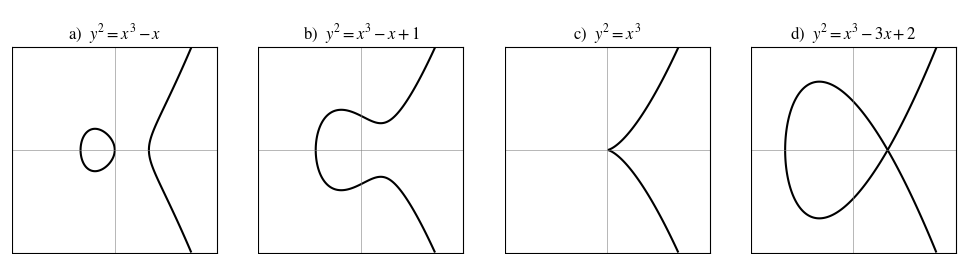
\includegraphics[width=0.8\textwidth]{img/elliptic_curves}
    \caption{Możliwe kształty krzywych eliptycznych w \( \real^2 \)}
    \label{fig:elliptic_curves}
\end{figure}

\subsection{Działania na krzywej eliptycznej}
Jeśli punkt \( P = (x, y) \) leży na krzywej eliptycznej, to \( -P = (x, -y) \) również.
Jeśli \( P \) i \( Q \) są punktami na krzywej eliptycznej, to prosta \( PQ \) przecina krzywą jeszcze w jednym punkcie \( R \).
Ustalamy, że \( P + Q + R = O \), gdzie \( O \) jest sztucznym punktem w nieskończoności. \\
\textit{(Niestety nie wiadomo, gdzie konkretnie jest \( O \) -- szczęśliwy znalazca proszony o kontakt.)}

\begin{figure}[H]
\centering
    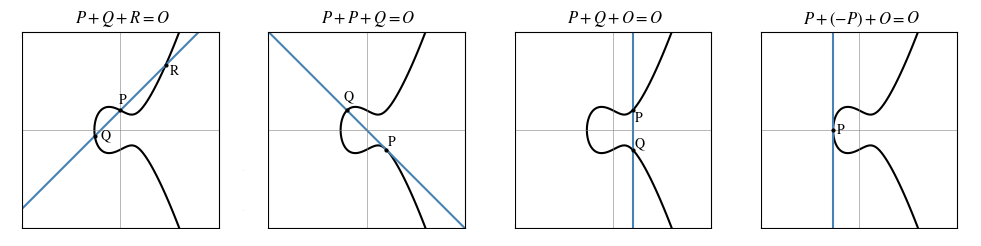
\includegraphics[width=0.8\textwidth]{img/elliptic_curves_lines}
    \caption{Możliwe przecięcia prostej z krzywą eliptyczną}
    \label{fig:elliptic_lines}
\end{figure}

Jeżeli \( Q = P \), traktujemy punkt \( P \) trochę jak podwójny pierwiastek wielomianu, który odbija się od osi, nie przecinając jej.
Za prostą \( PQ \) przyjmujemy wtedy styczną do krzywej w \( P \) (Rys.~\ref{fig:elliptic_lines}b).

Jeżeli \( Q = -P \), przyjmujemy, że \( P + Q = P + (-P) = O \) oraz \(P + O = P \) (Rys.~\ref{fig:elliptic_lines}c).

Podsumowując:
\begin{definition}[Dodawanie]
    Jeśli \( P \), \( Q \) są punktami na krzywej eliptycznej, to punkt \( R \) przecięcia prostej \( PQ \) z krzywą daje wynik dodawania \( P + Q = -R \).
    Jeśli prosta \( PQ \) nie przecina krzywej w dodatkowym punkcie, to \( P + Q = O \).
\end{definition}

Ponieważ mnożenie wymaga stałej liczby operacji, to dla dowolnego punktu \( P \) oraz liczby \( k \) można obliczyć \( k \cdot P \) w \( \bigO(\log k) \) operacjach arytmetycznych w ciele, stosując coś w rodzaju szybkiego potęgowania.

\subsection{Grupa krzywej eliptycznej}
Dodawanie punktów na krzywej jest przemienne i (co nieoczywiste) łączne, więc otrzymujemy grupę przemienną z elementem neutralnym \( O \).

Najczęściej używa się krzywych:
\begin{itemize}
    \item nad \( \integer_p \), gdzie \( p \) jest dużą liczbą pierwszą,
    \item nad ciałem \( \text{GF}(2^s) \).
\end{itemize}

\begin{theorem}
    Niech \( \mathbb{F} \) będzie ciałem, \( \abs{\mathbb{F}} = q \) oraz niech \( E \) będzie grupą dla pewnej krzywej eliptycznej nad \( \mathbb{F} \). Grupa \( E \) jest albo grupą cykliczną, albo produktem dwóch grup cyklicznych.
\end{theorem}
Niech pozostanie bez dowodu.

Rozmiar grupy \( \abs{E} \) może być rozumiany jako liczba rozwiązań równania opisującego krzywą.
Dla połowy \( x \in \mathbb{F} \) wartość \( x^3 + ax + b \) jest resztą kwadratową, a wtedy odpowiadają jej dwa możliwe \( y \), więc punktów powinno być blisko \( q \).